\documentclass{article}
\usepackage[margin=0.5in]{geometry}
\usepackage[utf8]{inputenc}
\usepackage{subcaption}
\usepackage{amsmath}
\usepackage{graphicx}
\usepackage{gensymb}

\graphicspath{ {img/} }
\title{Ant Speed Scratch Work}
\author{Matthew Moreno}

\usepackage{mathtools}
\DeclarePairedDelimiter\norm{\lVert}{\rVert}%

\begin{document}
\maketitle

\section{Discussion}

Calculating proper ant speed when the ant's heading is aligned with the gradient of a surface (i.e. the ant is traveling directly up a simple ramp) is straightforward.
Figure \ref{fig:ant_straight} depicts this scenario.
Thanks to the work of some poor biologists measuring ants walking up and down a tube, the walking speed of an ant traveling in parallel with the gradient of a simple ramp with incline $\gamma$ can be figured by consulting \cite[Figure 2B]{Holt2012LocomotionTerrain}.
(Note that this is speed relative to the surface the ant is traversing.
To figure speed relative to a horizontal x-y plane, divide by $\cos(\gamma)$.)

When the ant's heading is not aligned with the gradient of a surface, calculating the ant's walking speed becomes trickier. 
This scenario is depicted in Figure \ref{fig:ant_notstraight}.
The work done by \cite{Holt2012LocomotionTerrain}.
Last summer, to get a basic approximation, I worked with the ``effective incline'' $\dot{\gamma}$ that the ant was traversing.
I defined the effective incline as the inclination angle of a simple ramp where an ant would experience the ratio of distance traveled horizontally to distance traveled vertically while traveling parallel with the gradient of that simple ramp equivalent to the ratio of distance traveled horizontally to distance traveled vertically on its current trajectory.
As shown in Section \ref{sec:derivation}, the effective incline is calculated as
\begin{align} \label{eqn:effectiveincline}
\dot{\gamma} = \arctan{(\nabla S \cdot \hat{\vec{v}})},
\end{align}
where $\nabla S$ is the gradient of the surface that the ant is traversing and $\hat{\vec{v}}$ is the ant's normalized velocity (i.e. its heading with unit magnitude).

Now, there are two issues with this approach.
First is realism.
\cite{Holt2012LocomotionTerrain} hypothesize that ants maintain constant metabolic power output and their different walking speeds at different inclines result, in part, from different mechanical efficiencies of their gait depending on the incline they are traversing.
\cite{Holt2012LocomotionTerrain} measured ants walking in parallel with the gradient of a simple incline.
It is likely that the ants walking nonparallel with the gradient of a simple incline would suffer a different mechanical efficiency of their gait even if they were experiencing identical effective incline $\dot{\gamma}$.
For example, consider an ant walking on a flat surface and an ant walking directly across a simple ramp (perpendicular to the gradient). 
The ants experience identical effective incline $\dot{\gamma} = 0$ but mechanically are experiencing different gaits.
The ant on the flat surface has all six of its feet in the same vertical plane.
The ant traversing the simple ramp has its three feet on one side elevated above its three feet on the other.
My money would be on the ant on the flat surface enjoying a more efficient gait.
Unfortunately, the experiments performed by \cite{Holt2012LocomotionTerrain} only considered ants traveling in parallel to the gradient so there is not an obvious way to account for how mechanical efficiency of an ant's gait might depend on factors beyond the effective incline it is suffering.
It would be great to (a) concoct a clever \textit{in vivo} experiment to answer this question and then (b) convince someone to do it, but I doubt that's in the cards for the near future.
The second problem is numerical.
Calculations made using this approach won't be defined for vertical inclines (i.e. a wall with $90 \degree$ incline) or if the ant has no heading (i.e. zero velocity).
Numerical approximations will be hokey near these undefined cases.

At this point, using ``effective incline'' we have collapsed all possible ant headings relative to a surface's gradient to a roughly equivalent scenario where the ant is directly aligned with a surface's gradient.
Now, the question remains of how to determine the proper velocity of an ant given the effective incline it is suffering.
To answer this question, I used some heuristics to describe a relationship between $\dot{\gamma}$ and $\norm{\vec{v}}$.
This heuristic approach neglects formal consideration of units (i.e. rigorous physics).
I figured that there would be two major components determining the amount of power that an ant has to expend to walk on an incline.
First, the ant has to raise/lower its body vertically against the force of gravity (i.e. along the lines of raising/lowering a steel ball between the top/bottom of a cliff in intro physics).
It seemed reasonable that this component of the ant's expenditure might be proportional to $\sin{(\dot{\gamma})}) \times \norm{\vec{v}}$.
Second, the ant has to deal with mechanical inefficiencies in its gait.
It seemed reasonable that this component of the ant's expenditure might be proportional to $\norm{\vec{v}}^2$.
Based on the observations of \cite{Holt2012LocomotionTerrain}, this mechanical inefficiency expenditure seems to increase as the ant experiences effective inclines that are steeper (both upwards or downwards) than 0.
Scaling this expenditure by $[\texttt{incline\_scale} - \cos{(\dot{\gamma})}]$ where $\texttt{incline\_scale} > 1$ seemed like a computationally tractable way to account for this observation.

Putting these components together yields the expression,
\begin{align} \label{eqn:powerrelationship}
\texttt{ant\_power} 
&= \norm{v}^2[\texttt{incline\_scale} - \cos{(\dot{\gamma})}] + \texttt{gravity\_scale} \times \sin{(\dot{\gamma})} \times \norm{v}.
\end{align}
Fitting the coefficients to data points guesstimated from \cite{Holt2012LocomotionTerrain} | as depicted on 
Slide 15, Figure 10 of \texttt{extended-final-presentation.pdf} | yielded $\texttt{power} = 0.8115$, $\texttt{incline\_scale} = 1.2144$, $\texttt{gravity\_scale} = 0.2005$.

Now, we have a relationship between $\norm{\vec{v}}$ and the ant's heading relative to the surface ($\nabla S \cdot \hat{\vec{v}}$).
Let's solve out for $\hat{\vec{v}}$.
Substituting Expression \ref{eqn:effectiveincline} into Equation \ref{eqn:powerrelationship},
\begin{align*}
\texttt{ant\_power}
&= \norm{v}^2[\texttt{incline\_scale} - \cos{(\arctan{(\nabla S \cdot \hat{\vec{v}})})}] + \texttt{gravity\_scale} \times \sin{(\arctan{(\nabla S \cdot \hat{\vec{v}})})} \times \norm{v}.
\end{align*}
Noting that $\cos{(\arctan{(x)})} = \frac{1}{\sqrt{1 + x^2}}$ and $\sin{(\arctan{(x)})} = \frac{x}{\sqrt{1 + x^2}}$, we simplify 
\begin{align*}
\texttt{ant\_power}
&= \norm{v}^2 \Big[\texttt{incline\_scale} - \frac{1}{\sqrt{1 + (\nabla S \cdot \hat{\vec{v}})^2}}\Big] + \texttt{gravity\_scale} \times \frac{\nabla S \cdot \hat{\vec{v}}}{\sqrt{1 + (\nabla S \cdot \hat{\vec{v}})^2}} \norm{v}
\end{align*}
Equivalently,
\begin{align*}
0
&= \norm{v}^2 \Big[\texttt{incline\_scale} - \frac{1}{\sqrt{1 + (\nabla S \cdot \hat{\vec{v}})^2}}\Big] + \texttt{gravity\_scale} \times \frac{\nabla S \cdot \hat{\vec{v}}}{\sqrt{1 + (\nabla S \cdot \hat{\vec{v}})^2}} \norm{v} - \texttt{ant\_power}
\end{align*}
Using the quadratic formula, we can solve out for $\norm{v}$,
\begin{align*}
\norm{v} &= \frac{-b\pm\sqrt{b^2-4ac}}{2a},
\end{align*}
where $a = \Big[\texttt{incline\_scale} - \frac{1}{\sqrt{1 + (\nabla S \cdot \hat{\vec{v}})^2}}\Big]$, $b = \texttt{gravity\_scale} \times \frac{\nabla S \cdot \hat{\vec{v}}}{\sqrt{1 + (\nabla S \cdot \hat{\vec{v}})^2}}$, and $c = - \texttt{ant\_power}$.
At this point, some further simplifications can be made to streamline computation, but those are neglected here.


\begin{figure}
    \centering
    \begin{subfigure}[t]{0.4\textwidth}
        \centering
        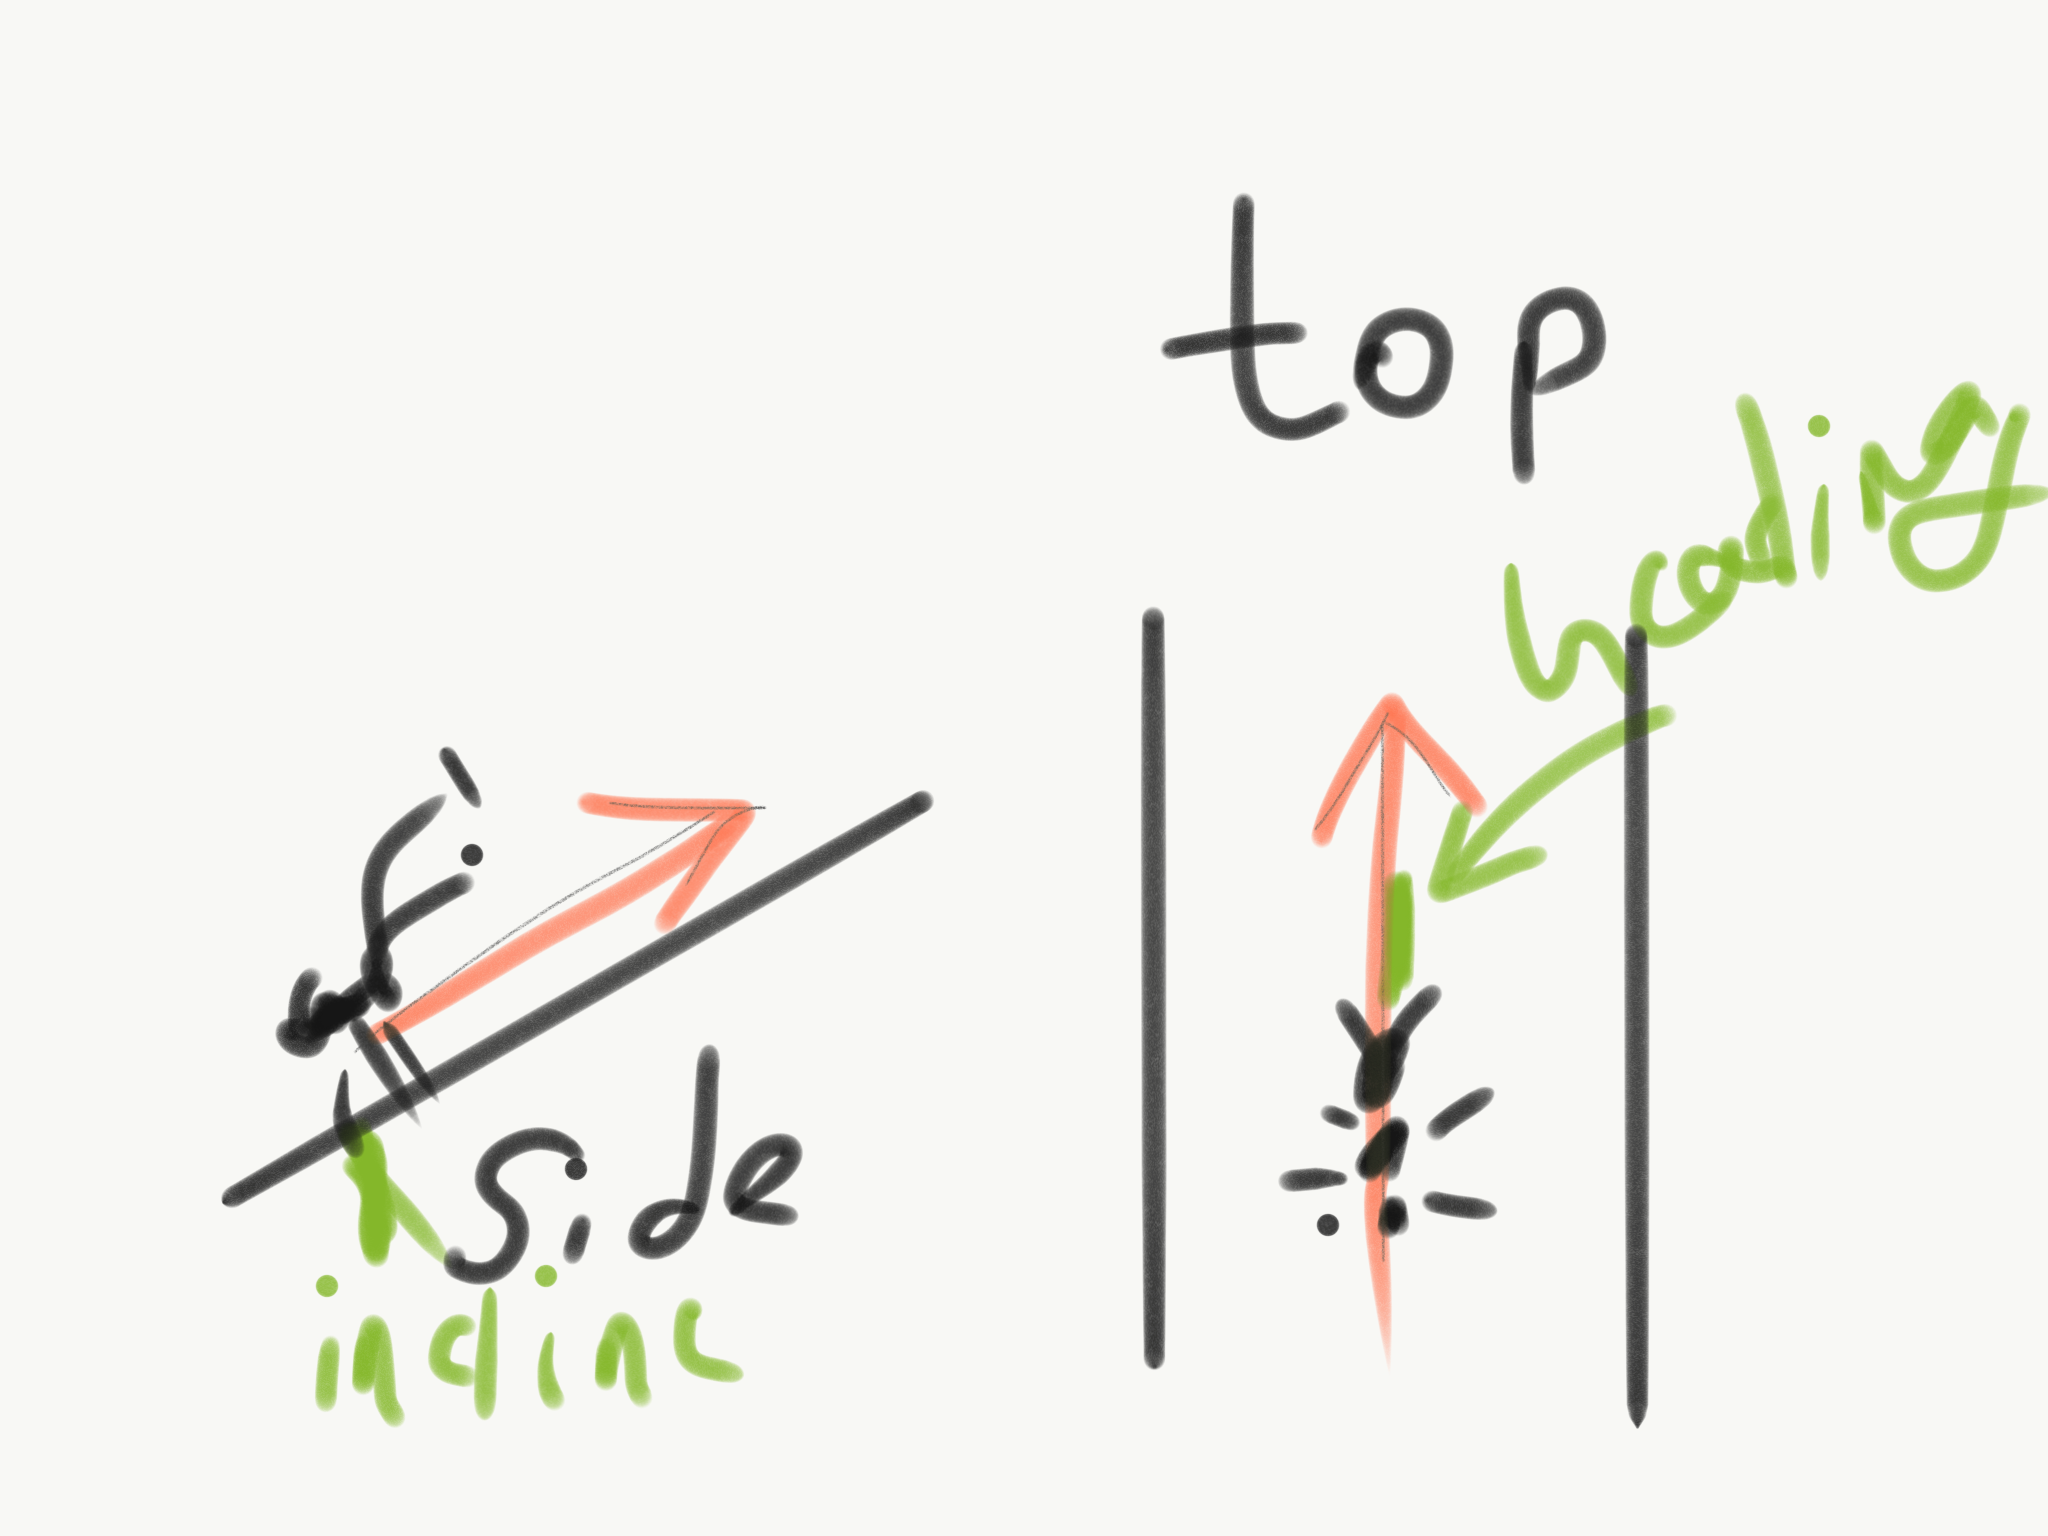
\includegraphics[height=2in]{ant_straight}
        \caption{Depiction of an ant traversing a simple incline with a heading parallel to the gradient of the incline.}
        \label{fig:ant_straight}
    \end{subfigure}
    \begin{subfigure}[t]{0.4\textwidth}
        \centering
        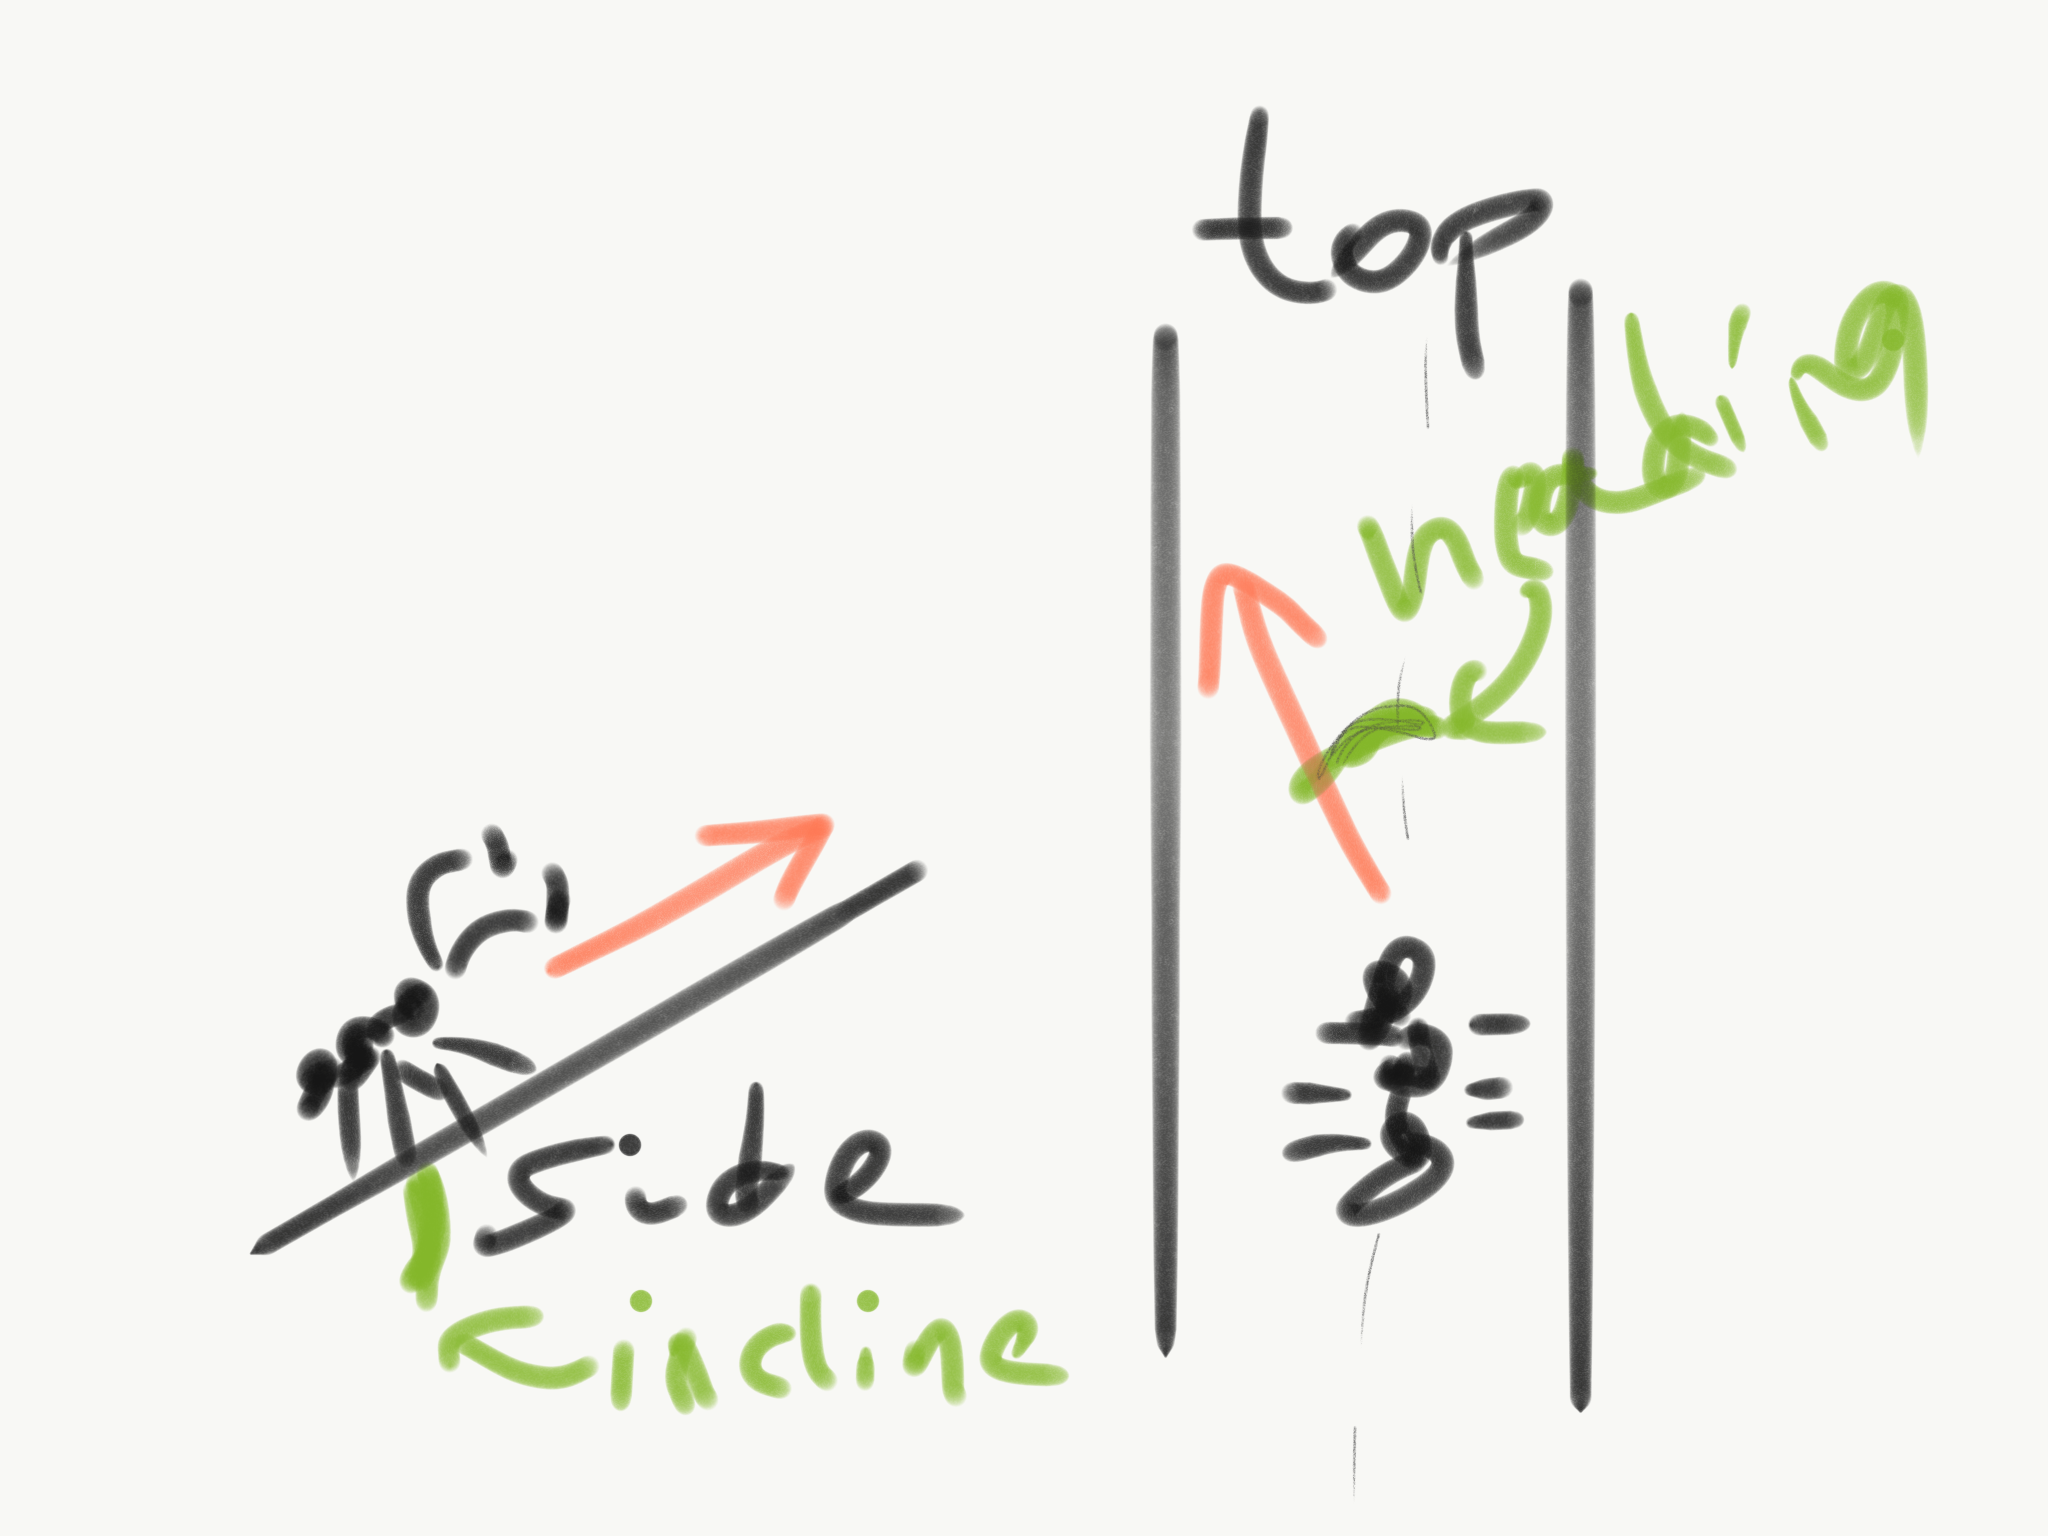
\includegraphics[height=2in]{ant_notstraight}
        \caption{Depiction of an ant traversing a simple incline with a heading askew from the gradient of the incline.}
        \label{fig:ant_notstraight}
    \end{subfigure}
    \caption{Schematics illustrating ant incline and heading.}
    \label{fig:ant_incline_heading}
\end{figure}

\section{Derivation} \label{sec:derivation}

The gradient of a two dimensional surface $S(x,y)$ is defined as
\begin{align*}
\nabla S = \begin{bmatrix}
           \frac{\delta S}{\delta x}  \\
           \frac{\delta S}{\delta y}
         \end{bmatrix}.
\end{align*}
The velocity of an ant is given as
\begin{align*}
\vec{v} = \begin{bmatrix}
           \frac{\delta x}{\delta t}  \\
           \frac{\delta y}{\delta t}
         \end{bmatrix}.
\end{align*}
Let us consider the normalized (i.e. unit vector) velocity of an ant, $\hat{\vec{v}}$, as the heading of that ant. 
We can figure the rate of ascension of the ant (i.e. altitude gained vertically per unit time) as
\begin{align*}
\frac{d S}{d t} \times 
&= \frac{\delta S}{\delta x} \times \frac{\delta x}{\delta t} + \frac{\delta S}{\delta y} \times \frac{\delta y}{\delta t} \\
&= \nabla S \cdot \vec{v}.
\end{align*}
The ratio of distance traveled vertically (i.e. altitude gained vertically) to distance traveled horizontally (i.e. in the x-y plane) is given as
\begin{align*}
\frac{\frac{d S}{d t}}{\norm{\vec{v}}} 
&= \frac{ \nabla S \cdot \vec{v}}{\norm{\vec{v}}} \\
&= \nabla S \cdot \hat{\vec{v}}
\end{align*}
Note that $\norm{\vec{v}}$ represents the distance traveled by ant in the x-y plane per unit time.
From here, we can calculate the effective angle of inclination, $\dot{\gamma}$, the ant is suffering.
\begin{align*}
\tan{(\dot{\gamma})} = \nabla S \cdot \hat{\vec{v}} \\
\dot{\gamma} = \arctan{(\nabla S \cdot \hat{\vec{v}})}
\end{align*}

 \bibliography{Mendeley}
 \bibliographystyle{apalike}

\end{document}
